%
% higherdim.tex -- XXX
%
% (c) 2019 Prof Dr Andreas Mueller
%
\section{Characteristics in higher dimensions}
\rhead{Characteristics in higher dimensions}
We now want to study the questions of characteristics in higher dimensions.
Characteristics seem to have to do something with the propagation of
waves, the characteristic curves in the twodimensional examples indicated
waves travelling in two directions.
In three dimensions, we expect a wave to travel as growing circles away from
the origin of the wave, describing a cone in threedimensional space.
So the natural generalization of the characteristic curves will be
surfaces.
To keep the discussion simple enough we restrict ourselves to the
three-dimensional case.

\subsection{The problem}
The Cauchy problem for a partial differential equation of the form
\[
\sum_{i,j=1}^3a_{ij}\partial_i\partial_ju+\sum_{i=1}^3b_i\partial_iu+cu=f
\]
is to prescribe the values of $u$ and first derivatives on a surface,
which may be specified as
\[
\omega(x_1,x_2,x_3)=0.
\]
Only the derivative in a direction orthogonal to the surface adds
new information.
It can be computed using the gradient
\[
\frac{\partial u}{\partial n}=\operatorname{grad}u\cdot \frac{\operatorname{grad}\omega}{|\operatorname{grad}\omega|}.
\]
We would like to understand under what conditions this initial data
determines the solution uniquely.

\subsection{A special case\label{subsection:a-special-case}}
We consider the special case where initial values are specified on the
plane $x_1=0$, i.~e.
\begin{align*}
u(0,x_2,x_3)&=u_0(x_2,x_3),
\\
\partial_1u(0,x_2,x_3)&=h(x_2,x_3).
\end{align*}
This corresponds to the case $\omega(x_1,x_2,x_3)=x_1$.

By prescribing initial values via a function $u_0$ on the plane $x_1=0$,
the first partial derivatives $\partial_iu$ for $i=2,3$ are already fixed,
they can be obtained by taking the partial derivatives of $u_0$
with respect to $x_2,\dots,x_3$.
If the partial derivative $\partial_1 u$ is also prescribed on the border,
then all the second second order derivatives
\[
\partial_i\partial_ju(0,x_2,x_3)\qquad 2\le i\le 3,\;1\le j\le 3
\]
are also known, we can obtain them by takeing derivatives of the
boundary conditions with respect to $x_2$ and $x_3$.
So the only second order derivative not yet known is $\partial_1^2u$.
Whether or not the partial differential equation determines the solution
uniquely thus hinges on the whether or not the equation determines
this second order derivative uniquely.

We can solve the partial differential equation for $\partial_1^2u$
if $a_{11}\ne 0$.
This is equivalent to
\[
a_{11}=\begin{pmatrix}
1&0&\dots&0
\end{pmatrix}
A
\begin{pmatrix}1\\0\\\vdots\\0\end{pmatrix}
=0.
\]

\subsection{The general case\label{subsection:the-general-case}}
We consider the function
$\omega(x_1,x_2,x_3)$
as representing the first coordindate of a new coordinate system.
We call the coordinates of this new system
$\omega_1,\dots,\omega_3$,
they are functions of the old coordinates as in
\[
\omega_1(x_1,x_2,x_3)=\omega(x_1,x_2,x_3)
,\qquad
\omega_2(x_1,x_2,x_3)
,\qquad
\omega_3(x_1,x_2,x_3).
\]
The function $u$ can also be written in these new coordinates,
we denote it as $\tilde u(\omega_1,\omega_2,\omega_3)$.
$\tilde u$ has the property
\[
\tilde u(
\omega_1(x_1,x_2,x_3),
\omega_2(x_1,x_2,x_3),
\omega_3(x_1,x_2,x_3)) = u(x_1,x_2,x_3).
\]
Substituting this into the partial differential equation, we obtain
\begin{align*}
\partial_iu
&=
\sum_{k=1}^3
\frac{\partial\tilde u}{\partial \omega_k}
\frac{\partial\omega_k}{\partial x_i}
\\
\partial_i\partial_ju
&=
\sum_{k,l=1}^3
\frac{\partial^2\tilde u}{\partial \omega_k\partial\omega_l}
\frac{\partial\omega_k}{\partial x_i}
\frac{\partial\omega_l}{\partial x_j}
\\
\sum_{i,j=1}^3a_{ij}\partial_i\partial_ju
&=
\sum_{i,j,k,l=1}^3a_{ij}
\frac{\partial^2\tilde u}{\partial \omega_k\partial\omega_l}
\frac{\partial\omega_k}{\partial x_i}
\frac{\partial\omega_l}{\partial x_j}
\\
\sum_{i=1}^3b_i\partial_iu
&=
\sum_{i,k=1}^3b_i
\frac{\partial\tilde u}{\partial \omega_k}
\frac{\partial\omega_k}{\partial x_i},
\end{align*}
thus the partial differential equation for $\tilde u$ in the
new coordinates is
\[
\sum_{k,l=1}^3a_{ij}
\biggl(
\sum_{i,j=1}^3a_{ij}
\frac{\partial\omega_k}{\partial x_i}
\frac{\partial\omega_l}{\partial x_j}
\biggr)
\frac{\partial^2\tilde u}{\partial \omega_k\partial\omega_l}
+
\sum_{k=1}^3
\biggl(
\sum_{i=1}^3
b_i
\frac{\partial\omega_k}{\partial x_i}
\biggr)
\frac{\partial\tilde u}{\partial \omega_k}
+c\tilde u
=f.
\]
The new coefficients of the second order derivatives are
\[
\tilde a_{kl}=
\sum_{i,j=1}^3a_{ij}
\frac{\partial\omega_k}{\partial x_i}
\frac{\partial\omega_l}{\partial x_j}.
\]
In $\omega$-coordinates, the Cauchy initial surface is described by
the equation $\omega_1=0$, so we have reduced the general case
to the special case of section~\ref{subsection:a-special-case}.
We conclude that the second order derivative is determined by the
partial differential equation from initial conditions if the 
coefficient $\tilde a_{11}$ does not vanish.
Thus not all the second order derivatives are determined if
\[
\sum_{i,j=1}^3
a_{ij}
\frac{\partial\omega}{\partial x_i}
\frac{\partial\omega}{\partial x_j}
=
\operatorname{grad}\omega
\cdot
A
\operatorname{grad}\omega
=0.
\]
As the gradient is orthogonal to the surface, we have found that a
surface is problematic if the the normal vector $\vec{n}$ satisfies
the vector equation
\[
\vec n\cdot A\vec n=0.
\]
These vectors are called {\em characteristic normals}.
\index{characteristic normals}

\begin{definition}
A surface defined by the equation
$\omega(x_1,\dots,x_n)=0$
is called {\em characteristic surface} if 
\[
\sum_{i,j=1}^na_{ij}\partial_i\omega\partial_j\omega=0
\]
everywhere on the surface.
\end{definition}

\subsection{Characteristic surfaces of the wave equation}
\begin{figure}
\begin{center}
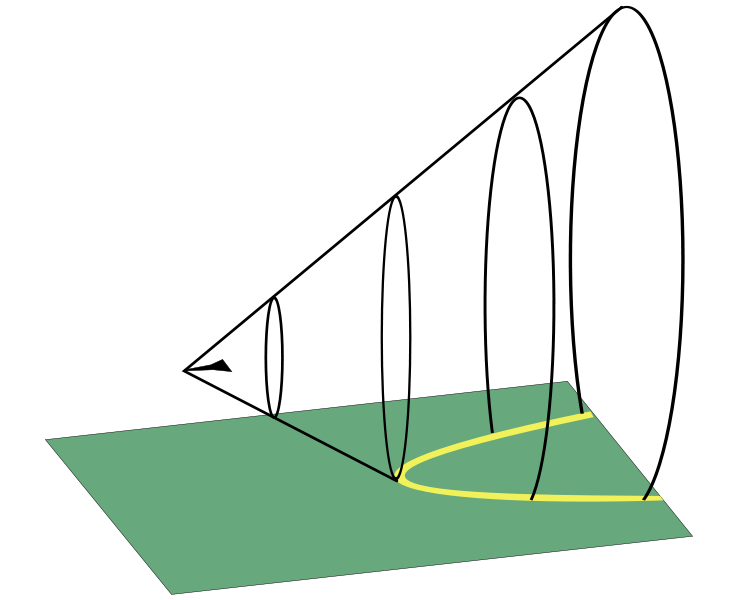
\includegraphics[width=0.8\hsize]{../common/graphics/shock}
\end{center}
\caption{Shock wave of a supersonic plane as an example of a characteristic
surface of the wave equation
$\partial_t^2u-a^2\Delta u=0$.\label{ueberschallkegel}}
\end{figure}
We determine the characteristic surfaces for the standard wave equation
\[
\partial_t^2u-a^2\Delta u=0.
\]
The coefficient matrix is
\[
A=\begin{pmatrix}
1&0&0\\
0&-a^2&0\\
0&0&-a^2
\end{pmatrix},
\]
thus the characteristic normals are vectors $\vec{v}$ that satisfy
the equation
\[
v_1^2-a^2v_2^2-a^2v_3^2
=
v_1^2 - a^2 (v_2^2+v_3^2)
=
0.
\]
These describe a double cone.
All vectors that have a fixed angle to the $x_1$ axis are characteristic
normals.
The angle $\alpha$ is subject to the condition
\[
\cos^2\alpha-a^2\sin^2\alpha=0,
\]
from which we derive
\[
\tan\alpha=\pm\frac1a.
\]

This angle condition is the only restriction for a characteristic surface.
Accordingly, there is a great variety of surfaces:
\begin{enumerate}
\item
Any cone with a opening angle
$\frac{\pi}2-\alpha$
and axis parallel to the $x_1$-axis is a characteristic surface.
The cone intersects the
$x_2$-$x_3$-plane in a circle with a radius that grows with velocity $a$
when $x_1$ increases.

Figure~\ref{ueberschallkegel} shows the shock wave produced by a
supersonic plane.
Shock waves as discontinuities of the solution must propagate along
characteristic surfaces, so they must form such a cone.
\item 
Ever plane a an angle of $\frac\pi2-\alpha$ to the $x_1$-axis
is a characteristic surface.
Such a plane intersects the $x_2$-$x_3$-plane in a straight line
that moves with velocity $a$ orthogonal to the straight line.
It describes a plane wave.

\end{enumerate}


